%!TEX root = ../../../adrien_gomar_phd.tex

\begin{figure}[htp]
  \centering
  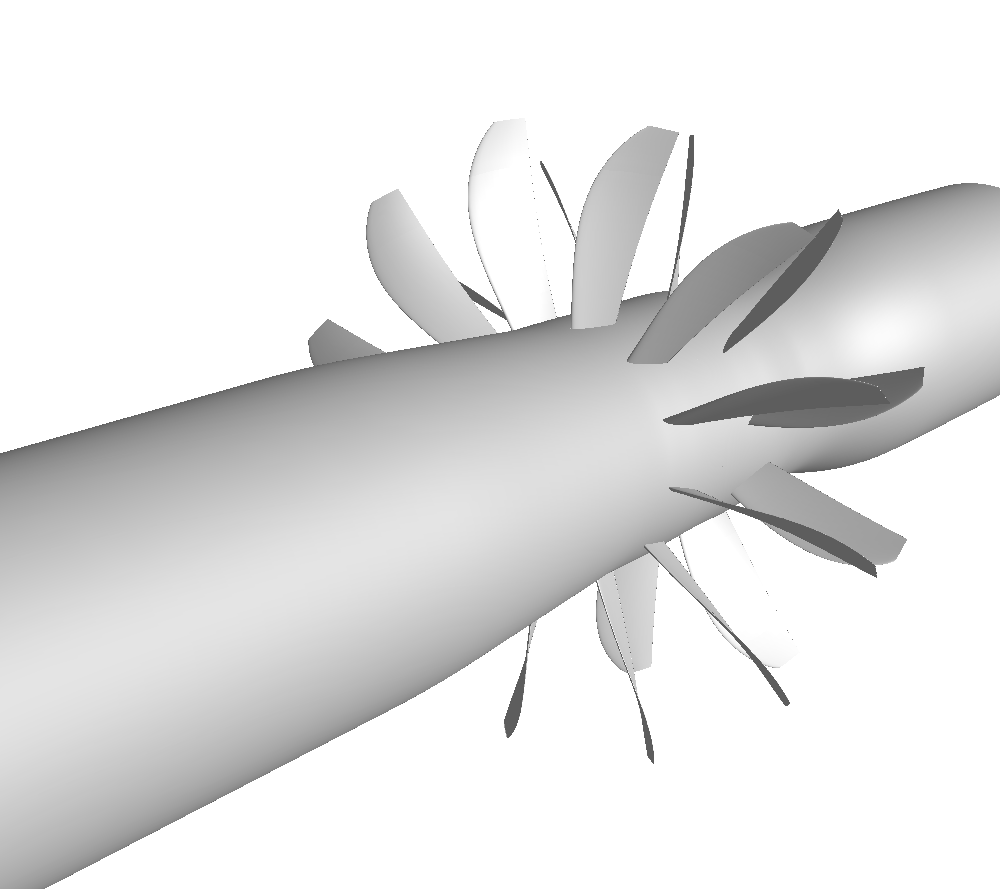
\includegraphics[width=.3\textwidth]{DREAM_HS_wall.png}
  \caption{High-speed isolated contra-rotating open rotor geometry.}
  \label{fig:dream_hs_wall}
\end{figure}

The configuration studied in this chapter is the same as the
one studied in the preceding Chapter but the blades have a 
different staggering angle. The geometry is shown in Fig.~\ref{fig:dream_hs_wall}.
In fact, this CROR is the High-Speed (HS) version of the previous one, 
representative of the cruise flight condition. The rotation speed being kept
almost constant between the two configuration, the only way to ensure
the proper adaptation of the flow field is to change the angle of 
attack of each section of the blade.

The main input parameters of the case are recalled in
Tab.~\ref{tab:dream_hs_flight_condition}.
\begin{table}[htp]
  \ra{1.3} \centering
  \begin{tabular}{cccc}
    \toprule
    $M_0$ & $|\Omega|$ & $J$ & $M_{tip}$ \\
    \midrule
    $0.73$ & $6057$ tr.min\textsuperscript{-1} & 3.7 & 0.96  \\
    \bottomrule
  \end{tabular}
  \caption{High-speed isolated contra-rotating open rotor flight condition parameters.}
  \label{tab:dream_hs_flight_condition}
\end{table} 
The inflow Mach number is within the transonic range. Its high value
can suggest shocks. This is emphasized by the $M_{tip}$ which is
near from being supersonic.
